% !TeX root = Report.tex
\documentclass[a4paper,12pt]{report}
% !TeX root = main.tex
%_______________________________ Packages ______________________________
\usepackage[utf8]{inputenc}
\usepackage[french]{babel}       %for language
\usepackage{float} %for H
\usepackage{blindtext}                                                  %for Dummy Text
\usepackage[a4paper,top=2.5cm,bottom=2.5cm,left=2.75cm,right=2.75cm]{geometry}    %for document shape
\usepackage{graphicx}                                                   %images
\usepackage{enumitem}                                                   % Used to compact lists
\usepackage{fancyhdr}                                                   %fancy headers
\usepackage{amsmath}                                                    %maths
\usepackage{titling}                                                    %for a pretitle f maketitle
\usepackage{tikz}
\usepackage{fancybox}
\usepackage{tabularx}
\usepackage{wrapfig}
\usepackage{titlesec}
\usepackage{hyperref}
\usepackage{indentfirst}
\usepackage[footnote]{acronym}
\usepackage{eurosym}

%_______________________________________________________________________
%_______________________________ for font ______________________________
%\renewcommand{\familydefault}{\sfdefault}     
\selectlanguage{french}
%_______________________________________________________________________
%___________________________ for fancy pages ___________________________
\pagestyle{fancy}   
\renewcommand{\headrulewidth}{1pt}
\renewcommand{\footrulewidth}{1pt}
\fancyhead[R,L]{\chaptername \  \thechapter}
\fancyhead[LE,RO]{\rightmark} 
\addto\captionsenglish{% Replace "english" with the language you use
  \renewcommand{\contentsname}%
    {Table des matières}%
}

 %%%%********************************************************************
\definecolor{quotemark}{gray}{0.7}
\makeatletter
\def\fquote{%
    \@ifnextchar[{\fquote@i}{\fquote@i[]}%]
           }%
\def\fquote@i[#1]{%
    \def\tempa{#1}%
    \@ifnextchar[{\fquote@ii}{\fquote@ii[]}%]
                 }%
\def\fquote@ii[#1]{%
    \def\tempb{#1}%
    \@ifnextchar[{\fquote@iii}{\fquote@iii[]}%]
                      }%
\def\fquote@iii[#1]{%
    \def\tempc{#1}%
    \vspace{1em}%
    \noindent%
    \begin{list}{}{%
         \vspace{3.6cm}
         \setlength{\leftmargin}{0.1\textwidth}%
         \setlength{\rightmargin}{0.1\textwidth}%
                  }%
         \item[]%
         \begin{picture}(0,0)%
         \put(-15,-5){\makebox(0,0){\scalebox{3}{\textcolor{quotemark}{``}}}}%
         \end{picture}%
         \begingroup\itshape}%
 %%%%********************************************************************
 \def\endfquote{%
 \endgroup\par%
 \makebox[0pt][l]{%
 \hspace{0.8\textwidth}%
 \begin{picture}(0,0)(0,0)%
 \put(15,15){\makebox(0,0){%
 \scalebox{3}{\color{quotemark}''}}}%
 \end{picture}}%
 \ifx\tempa\empty%
 \else%
    \ifx\tempc\empty%
       \hfill\rule{100pt}{0.5pt}\\\mbox{}\hfill\tempa,\ \emph{\tempb}%
   \else%
       \hfill\rule{100pt}{0.5pt}\\\mbox{}\hfill\tempa,\ \emph{\tempb},\ \tempc%
   \fi\fi\par%
   \vspace{0.5em}%
 \end{list}%
 }%
 \makeatother
 %%%%********************************************************************

\setcounter{secnumdepth}{4} % seting level of numbering (default for "report" is 3).

\bibliographystyle{plain}
\newenvironment{remerciements}
{%begin
    \begin{titlepage}
    \hspace{0pt}
    \vfill
    \begin{center}
        \textbf{\Large Remerciement}
    \end{center}
    \hrule\bigskip
}
{%end
    \begin{center}
        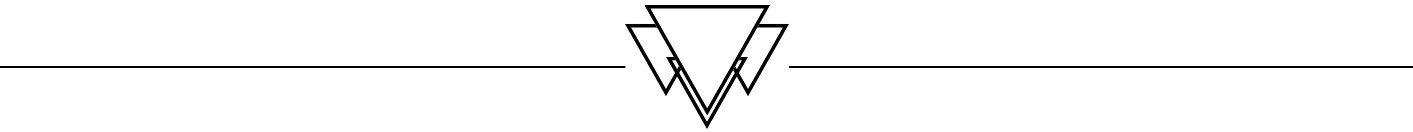
\includegraphics[width = \linewidth]{images/zwa9a line.png}
    \end{center}
    \vfill
    \hspace{0pt}
    \end{titlepage}
}


\newenvironment{resume}
{%begin
    
    \begin{titlepage}
    \hspace{0pt}
    \vfill
    \begin{center}
        \textbf{\Large Résumé}
    \end{center}
    \hrule\bigskip
}
{%end
    \begin{center}
        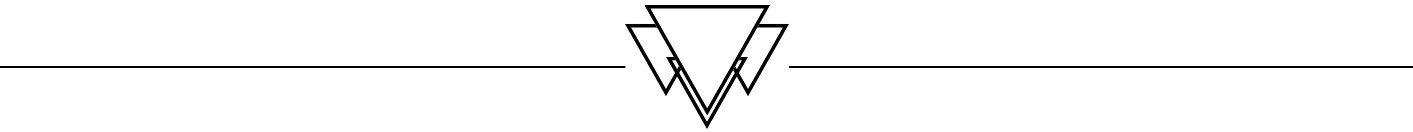
\includegraphics[width = \linewidth]{images/zwa9a line.png}
    \end{center}
    \vfill
    \hspace{0pt}
    \end{titlepage}
}

\newenvironment{englishabstract}
{%begin
    \begin{titlepage}
    \hspace{0pt}
    \vfill
    \begin{center}
        \textbf{\Large Abstract}
    \end{center}
    \hrule\bigskip
}
{%end
    \begin{center}
        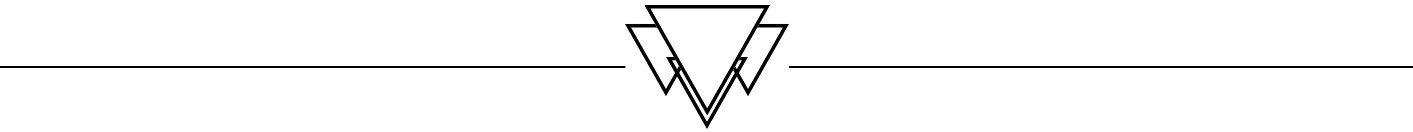
\includegraphics[width = \linewidth]{images/zwa9a line.png}
    \end{center}
    \vfill
    \hspace{0pt}
    \end{titlepage}
}



\newenvironment{introductiongenerale}
{%begin
    
    \begin{titlepage}
    \vspace*{1cm}
    \begin{center}
        \textbf{\Large Introduction Générale}
    \end{center}
    \hrule\bigskip
}
{%end
    \vfill
    \begin{center}
        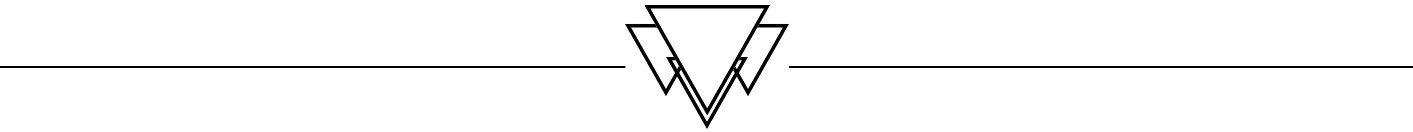
\includegraphics[width = \linewidth]{images/zwa9a line.png}
    \end{center}
    \vspace{3cm}
    \end{titlepage}
}

\newenvironment{conclusiongeneral}
{%begin
    
    \begin{titlepage}
    \vspace*{.5cm}
    \begin{center}
        \textbf{\Large Conclusion Finale}
    \end{center}
    \hrule\bigskip
}
{%end
    \vfill
    \begin{center}
        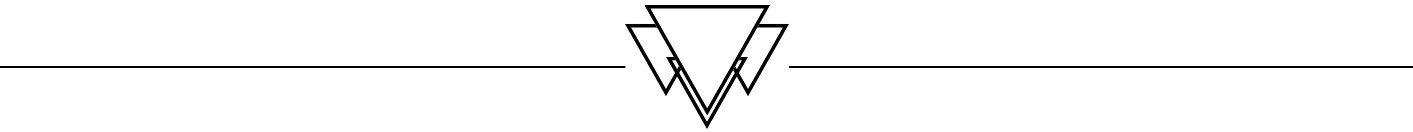
\includegraphics[width = \linewidth]{images/zwa9a line.png}
    \end{center}
    \vspace{3cm}
    \end{titlepage}
}


\begin{document}
    %================================COVER PAGE==============================
    \thispagestyle{empty} 
    \begin{titlepage}\label{TitlePäge}
\begin{center}
    \begin{figure}[!htb]
        \begin{minipage}{0.5\linewidth}
            
\includegraphics[width=0.58\linewidth]{logos/Um5-ENSIAS.png}
        \end{minipage}
        \hspace{1.8cm}
        \begin{minipage}{0.5\linewidth}
            
\includegraphics[width=0.84\linewidth]{logos/OBS.png}
        \end{minipage}
    \end{figure}
     
   \vspace*{1.6cm}

  \textsc{\huge \bfseries Projet de fin d'études}\\[1.3cm]
  \textsc{\small Filière}\\[1cm]
  \textsc{\huge \bfseries Génie Logiciel }\\[1.4cm]
  \textsc{\small Sujet}\\
  \begin{center}
 \rule{0.5\linewidth}{1pt}
 \end{center}
  \textsc{\huge \bfseries Automatisation des tests E2E et\\\vspace*{0.4cm} de non regression dans le cadre\\\vspace*{0.6cm} d’un projet de Monitoring }
  \begin{center}
 \rule{0.5\linewidth}{1pt}
 \end{center}
 
 \vspace{2.8cm}
  
  \begin{minipage}{0.5\textwidth}
    \vspace{-6mm}
  \begin{flushleft} \large
    \emph{\bfseries Réalisé par}\\[0.3cm]
    Yassine OUHADI \\[0.5cm]
    \emph{\bfseries Encadré par} \\[0.3cm]
    Mlle. EL KHAIR Chaimae - Ingénieure QA chez OBS
  \end{flushleft}
\end{minipage}
\begin{minipage}{0.4\textwidth}
  \begin{flushright} \large
    % \begin{flushleft} \large
    \emph{\bfseries Membres du jury} \\[0.3cm]
    Pr. A. El Hassouny - ENSIAS\\[0.3cm]
    Pr. W. Ettazi - ENSIAS \\
    % \end{flushleft}

  \end{flushright}
\end{minipage}\\[1cm]


  
  
  

  \vspace{0.4cm} 	
  \begin{center}
    {Année Universitaire 2024-2025}
  \end{center}

   \end{center}
\end{titlepage} 
    \cleardoublepage
    
    %================================Dedicace============================
    \newpage
    \begin{fquote}
\begin{center}
\thispagestyle{empty}
\large{

% \uppercase
\textbf{À mes chers parents,} dont l'amour et le soutien ont été inestimables, aucune déclaration de gratitude ne serait suffisante pour exprimer la profondeur de mon respect et de ma reconnaissance envers vous. Vos sacrifices et vos encouragements ont été les fondements de ma réussite éducative et personnelle.

\textbf{À mes amis et camarades étudiants de l'ENSIAS,} qui ont été une source constante de motivation et de soutien tout au long de mon parcours académique. Votre amitié et votre collaboration ont été essentielles dans mon développement.

\textbf{Au corps enseignant du département de génie logiciel,} je suis reconnaissant pour vos connaissances partagées, votre patience et vos conseils qui ont éclairé mon chemin académique.

À tous ceux qui ont contribué de près ou de loin à la réalisation de ce travail
\\[12pt]
Merci.
}
\end{center}
\bigskip
\medskip
\end{fquote}

\hspace*{\fill} \textbf{\textit{\large{- Yassine}}}

\clearpage

    %================================REMERCIEMENT============================
    \newpage
    \begin{remerciements}
\end{remerciements}

    %================================RESUME============================
    \newpage
    \begin{resume}
Ce rapport présente mon projet de fin d’étude axé sur l’automatisation des tests E2E et des tests de non-régression dans le contexte d’un projet de monitoring. Il met en évidence l’importance cruciale des tests à toutes les étapes du cycle de développement, en particulier les tests de non-régression, indispensables pour maintenir l’indépendance des différents modules de l’application. L’automatisation de ces tests est présentée comme une approche visant à réduire la charge de travail et à améliorer la détection des anomalies. Parallèlement, les tests E2E automatisés sont déployés pour vérifier le bon fonctionnement global de l’application et garantir la conformité aux exigences du cahier des charges ainsi qu’aux SLA. En outre, ce projet vise à favoriser une meilleure application des principes Agile dans le processus de développement, contribuant ainsi à une approche plus efficace et réactive dans le cadre du monitoring des systèmes.
\end{resume}

    %==================================ABSTRACT==============================
    %\begin{resume}
Ce rapport présente mon projet de fin d’étude axé sur l’automatisation des tests E2E et des tests de non-régression dans le contexte d’un projet de monitoring. Il met en évidence l’importance cruciale des tests à toutes les étapes du cycle de développement, en particulier les tests de non-régression, indispensables pour maintenir l’indépendance des différents modules de l’application. L’automatisation de ces tests est présentée comme une approche visant à réduire la charge de travail et à améliorer la détection des anomalies. Parallèlement, les tests E2E automatisés sont déployés pour vérifier le bon fonctionnement global de l’application et garantir la conformité aux exigences du cahier des charges ainsi qu’aux SLA. En outre, ce projet vise à favoriser une meilleure application des principes Agile dans le processus de développement, contribuant ainsi à une approche plus efficace et réactive dans le cadre du monitoring des systèmes.
\end{resume}

    %================================RESUME============================
    \newpage
    \input{intro/Liste des abréviation}
    
    \newpage
    %===============================PLAN============================
    {
        \thispagestyle{empty}
        \tableofcontents
        \thispagestyle{empty}
    }
    {
        \thispagestyle{empty}
        \listoffigures
        \thispagestyle{empty}
    }

    %===============================INTRODUCTION============================
    \begin{introductiongenerale}
WATCH Project, Testing, L'automatisation des tests, Les Objectifes, Report Structure
\end{introductiongenerale}

    \chapter{Contexte général du projet}

\section{Introduction}

\section{Organisme d’accueil}
\subsection{Presentation de l’organisme}
\subsection{Ecosystème Orange Business}
\subsection{Les portefeuilles B2B}
\subsection{L'annuaire des trains Safe}
\subsection{L'entity CTIO}
\subsection{Les Departments CTIO}
\subsection{Equipe WATCH}

\section{Watch Testing}
\subsection{Problématique}
\subsection{Motivations}

\section{Conclusion}
    \chapter{Approche du Projet WATCH}

\section{Introduction}

\section{Vision du Projet}

\subsection{Objectifs du Projet}

\subsection{Ingestion et transformation des données}

\subsection{Gestion des Règles de corrélation}

\subsection{Supervision des alerts}

\subsection{Les clients de Watch}

\section{Méthodologie de Travail}

\section{Rôles et Responsabilités}

\section{Architecture Technique}

\section{Cadre de Développement}

\subsection{Outils}

\subsection{Intégration et test}

\subsection{Déploiement}

\section{L'état d'avancement du projet}

\clearpage

\section{Processus de Test}

\section{Problématique}

\section{Motivations}

\section{Conclusion}

    \input{chapters/3.L’automatisation des tests}
    \chapter{Analyse et conception}

\section{Introduction}

\section{Conclusion}
    \chapter{Réalisation et résultats}

\section{Introduction}

\section{Conclusion}
    \chapter{Conduite du projet}

\section{Introduction}

\section{Conclusion}

    %===============================CONCLUSION============================
    \begin{conclusiongeneral}
Conclusion et perspectives
\end{conclusiongeneral}
    
    %===============================BIBLIOGRAPHY============================
    \bibliography{BIBLIOGRAPHY}
\end{document}
